\documentclass{beamer}

\usepackage{iftex}
% Pakete u.a. für die Darstellung von Umlauten/Sonderzeichen
\ifPDFTeX
   \usepackage[utf8]{inputenc}
   \usepackage[T1]{fontenc}
   \usepackage{lmodern}
\else
   \ifXeTeX
     \usepackage{xltxtra}
   \else 
     \usepackage{luatextra}
   \fi
   \defaultfontfeatures{Ligatures=TeX}
\fi

\usepackage{amsthm}

\newtheorem{exercise}{Exercise}

\usepackage{listings}

\usepackage{url}

\lstdefinelanguage{gf}
{
  morekeywords={abstract, flags, cat, fun, incomplete, concrete, of, open, in, lincat, lin, resource, param, oper, variants, table, interface, instance, def, data, lindef, printname,},
  sensitive=false,
  morecomment=[l]{--},
  morestring=[b]",
  stringstyle={\textit}
}
\lstset{basicstyle=\ttfamily}

\title{GF for Python Programmers}
\author{Herbert Lange}
\begin{document}
\begin{frame}
  \maketitle
\end{frame}
\begin{frame}{Disclaimer}
  \begin{itemize}
  \item This tutorial is work in progress, you are the first ones to enjoy(?!?) this
  \item I am not really a Python programmer myself but I am trying my best to understand the Python way of doing things
  \item I hope we can find some connections Python $\Leftrightarrow$ GF
  \item We use Python 3
  \item The slides and a extended tutorial can be found on \url{https://github.com/daherb/GF-for-Python-programmers}
  \end{itemize}
  \begin{center}
    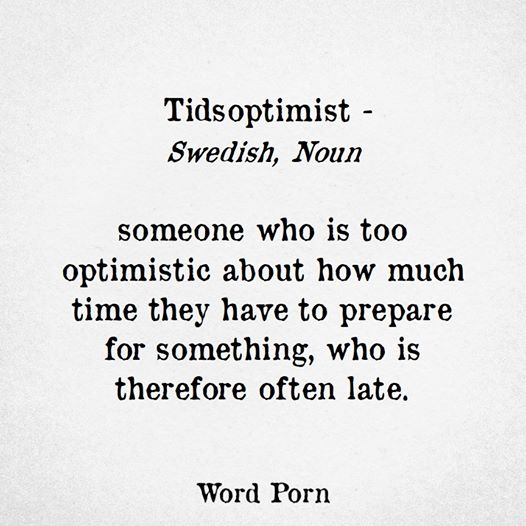
\includegraphics[height=10em]{tidsoptimist}
  \end{center}
\end{frame}

\begin{frame}{Types}
  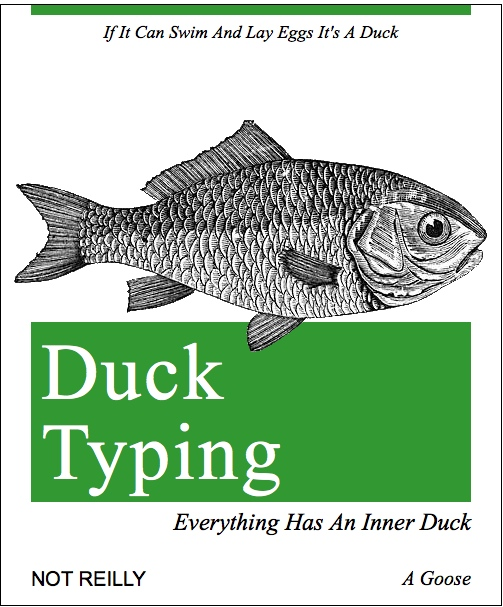
\includegraphics[height=10em]{types1}
  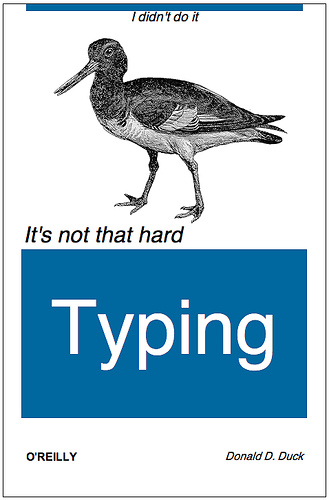
\includegraphics[height=10em]{types2}
  \begin{itemize}
  \item Python has types but people usually don't care too much about them
  \item But for GF types are important
  \item $\Rightarrow$ You should start to be aware of your types (especially for functions)
  \end{itemize}
\end{frame}
\begin{frame}{Types in Python 1}
 You can use the \texttt{type()} function to figure out the type of expressions in Python
 \begin{exercise}
   Fire up your Python shell and have a look at the types of some expressions.

   You can try 3, 3.0, ``Foo'', [1,2,3], (1,2,3), {'foo':1,'bar':2}, some defined variables, functions and lots of other things.
 \end{exercise}
\end{frame}
\begin{frame}{Types in Python 2}
  \begin{itemize}
  \item We can have basic types (e.g. numbers, strings, ...)
  \item compound or complex types (e.g. lists, tuples, dictionaries, ...)
  \item types by enumerating possible values
  \item functions
  \end{itemize}
  
\end{frame}

\begin{frame}[fragile]{Enumeration types}
  \begin{itemize}
  \item We can define new types by enumerate all possible values
  \item These values are mapped to e.g. integers
  \item We can use them to define e.g. grammatical features like number, case, gender, etc.
  \end{itemize}
\begin{verbatim}
>> class Number(Enum):
...   Sg = 1
...   Pl = 2
... 
>> type(Number.Sg)
<enum 'Number'>
\end{verbatim}
\end{frame}
\begin{frame}[fragile]{Dictionaries}
  \begin{itemize}
  \item Mapping from values of one type to values of another type
  \item Access values with the \texttt{[]} operator
  \end{itemize}
\begin{verbatim}
>>> man = {"s":{Number.Sg: "man" , Number.Pl: "men"}, 
           "g":Gender.Masc}
>>> man
{'g': <Gender.Masc: 1>, 
 's': {<Number.Pl: 2>: 'men', <Number.Sg: 1>: 'man'}}
>>> man["s"][Number.Sg]
'man'
\end{verbatim}
\end{frame}

\begin{frame}[fragile]
\begin{verbatim}
>>> class Case(Enum):
...   Nom = 1
...   Gen = 2
...   Dat = 3
...   Acc = 4
... 
>>> mann={Number.Sg:{Case.Nom:"Mann", 
...                  Case.Gen:"Mannes", 
...                  Case.Dat:"Mann", 
...                  Case.Acc:"Mann"},
...       Number.Pl:{Case.Nom:"Männer", 
...                  Case.Gen:"Männer", 
...                  Case.Dat:"Männern", 
...                  Case.Acc:"Männern"}
... }
>>> mann[Number.Sg][Case.Gen]
'Mannes'
\end{verbatim}
\end{frame}

\begin{frame}
  \begin{exercise}
Implement a function that takes a string of a noun and generates noun paradigms for English (or a language of your choice) as a dictionary of dictionaries. Also define all necessary grammatical features as enumeration types
\end{exercise}
\end{frame}
\begin{frame}[fragile]{Functions in Python}
  \begin{itemize}
  \item There are (at least) two ways to define functions in Python
  \item the most common one is to use \texttt{def} and give them a name directly
  \item but you can also define functions without names (anonymous functions)
  \end{itemize}
\begin{verbatim}
>>> def succ(x) :
...   return x+1
... 
>>> type(succ)
<class 'function'>
>>> succ2 = lambda x : x+1
>>> type(succ2)
<class 'function'>
>>> type(lambda x: x+1)
<class 'function'>
\end{verbatim}
\end{frame}

\begin{frame}
  \begin{exercise}
    Write some functions both as ``def''s and lambda expressions and try them on some parameters.

    You can try e.g. functions on strings.
  \end{exercise}
\end{frame}

\begin{frame}{Types in GF}
  Different types in abstract, concrete and resource modules:
  \begin{itemize}
  \item in abstract no types in the programming language sense, you can just see it as a kind of context free grammar with grammatical categories and syntax rules
  \item in resource modules we can use lots of types we already know from other languages
  \item in concrete syntax we can mostly focus on string tuples, records, tables and parametric types
  \end{itemize}
\end{frame}
\begin{frame}[fragile]
  \begin{lstlisting}
abstract Simple = {
  cat S ; NP ; VP ;
  fun
    sent : NP -> VP -> S ;
}
  \end{lstlisting}
  Here we can read it as a grammar with the three non-terminal symbols S, NP and VP and the one grammar rule equivalent to the CFG rule \texttt{S --> NP VP}
\end{frame}
\begin{frame}[fragile]
\lstinputlisting[language=gf]{../../src/SimpleTypes.gf}  
\begin{verbatim}
> cc s
"foobar"
0 msec
> cc st
"foo" ++ "bar"
0 msec
> cc succ i
43
0 msec
\end{verbatim}
\end{frame}

\begin{frame}{Tables and Records}
  \begin{itemize}
  \item GF knows both Tables and Records
  \item In Python both could be replaced with dictionaries (even there are also named tuples in Python)
  \item Tables are like the dictionaries where we used Enums as keys
  \item Records are like the dictionaries where we used strings as keys 
  \end{itemize}
\end{frame}

\begin{frame}[fragile]
Problem: Does not enforce totality
\begin{verbatim}
>>> mann={
...   Number.Sg:{
...     Case.Nom:"Mann"
...   },
...   Number.Pl:{
...     Case.Dat:"Männern"
...   }
... }
>>> mann[Number.Sg][Case.Gen]
Traceback (most recent call last):
  File "<stdin>", line 1, in <module>
KeyError: <Case.Gen: 2>
\end{verbatim}
GF does not allow that to happen. Tables have to be ``total'', i.e. there must be a mapping for all possible values (but we can use wildcards)
\end{frame}
\begin{frame}{Pattern matching}
  It is cool magic available in several programming languages but in python you need 3rd party modules

  Idea: e.g. if a noun ends in ``y'', then we replace it with ``ies'' to form the plural

  You can e.g. use pattern matching in \texttt{case} statements to implement nice smart paradigms
\end{frame}

\begin{frame}[fragile]
  \begin{lstlisting}
resource Res = {
  param Number = Sg | Pl ;
  oper
    Noun : Type = Number => Str;
    noun : Str -> Noun =
      \s -> table {
        Sg => s ; 
        Pl => case s of
             { 
               fl + "y" => fl + "ies" ;
               _ => s + "s"
             }
        } ;
}

  \end{lstlisting}
\end{frame}

\begin{frame}
  \begin{exercise}
    Write your own small smart paradigm. As an inspiration you can take the following German noun phrase
  \end{exercise}
\end{frame}

\begin{frame}[fragile]{GF in Python}
  \begin{itemize}
  \item Load pgf module
\begin{verbatim}
import pgf
\end{verbatim}
\item Load grammar
\begin{verbatim}
gr = pgf.readPGF("Foods.pgf")
\end{verbatim}
\item Parse sentence: Parsing is a funtion in the concrete syntax
\begin{verbatim}
eng = gr.languages["FoodsEng"]
i = eng.parse("this Italian pizza is very Italian")
p,e = i.__next__()
print(e)
\end{verbatim}
\item Generate trees: Generation is a function in the PGF grammar and linearization in the concrete syntax
\begin{verbatim}
i = gr.generateAll(gr.startCat)
p,e = i.__next__()
print(eng.linearize(e))
\end{verbatim}
  \end{itemize}
  Longer tutorial \url{http://www.grammaticalframework.org/doc/python-api.html}
\end{frame}
\begin{frame}
  \begin{exercise}
    If you have the Python module installed, try to load a grammar, parse a few sentences, generate a few trees, linearize trees, etc.
  \end{exercise}
\end{frame}
\end{document}
